\documentclass{beamer}
\usepackage[utf8]{inputenc}
\usepackage{graphicx, epsfig}
\usepackage{amsmath,mathrsfs,amsfonts,amssymb}
\usepackage{floatflt}
\usepackage{epic,ecltree}
\usepackage{mathtext}
\usepackage{fancybox}
\usepackage{fancyhdr}
\usepackage{multirow}
\usepackage{enumerate}
\usepackage{epstopdf}
\usepackage{multicol}
\usepackage{algorithm}
\usepackage[noend]{algorithmic}
\usepackage{tikz}
\usepackage{blindtext}
\usetheme{default}%{Singapore}%{Warsaw}%{Warsaw}%{Darmstadt}
\usecolortheme{default}

\setbeamerfont{title}{size=\Huge}
\setbeamertemplate{footline}[page number]{}

\setbeamertemplate{section in toc}[sections numbered]


\makeatletter
\newcommand\HUGE{\@setfontsize\Huge{35}{40}}
\makeatother    

\setbeamerfont{title}{size=\HUGE}
\beamertemplatenavigationsymbolsempty

% latin bold lower
\newcommand{\ba}{\mathbf{a}} 
\newcommand{\bc}{\mathbf{c}} 
\newcommand{\be}{\mathbf{e}} 
\newcommand{\bff}{\mathbf{f}} % \bf - for bold type
\newcommand{\bg}{\mathbf{g}} 
\newcommand{\bh}{\mathbf{h}} 
\newcommand{\bp}{\mathbf{p}} 
\newcommand{\bq}{\mathbf{q}} 
\newcommand{\bt}{\mathbf{t}} 
\newcommand{\bs}{\mathbf{s}} 
\newcommand{\bu}{\mathbf{u}} 
\newcommand{\bv}{\mathbf{v}} 
\newcommand{\bw}{\mathbf{w}} 
\newcommand{\bx}{\mathbf{x}} 
\newcommand{\by}{\mathbf{y}} 
\newcommand{\bz}{\mathbf{z}} 

% latin bold upper
\newcommand{\bA}{\mathbf{A}} 
\newcommand{\bB}{\mathbf{B}} 
\newcommand{\bC}{\mathbf{C}} 
\newcommand{\bG}{\mathbf{G}} 
\newcommand{\bI}{\mathbf{I}} 
\newcommand{\bJ}{\mathbf{J}} 
\newcommand{\bL}{\mathbf{L}} 
\newcommand{\bM}{\mathbf{M}} 
\newcommand{\bP}{\mathbf{P}}
\newcommand{\bQ}{\mathbf{Q}} 
\newcommand{\bR}{\mathbf{R}} 
\newcommand{\bT}{\mathbf{T}} 
\newcommand{\bU}{\mathbf{U}} 
\newcommand{\bV}{\mathbf{V}} 
\newcommand{\bW}{\mathbf{W}} 
\newcommand{\bX}{\mathbf{X}} 
\newcommand{\bY}{\mathbf{Y}} 
\newcommand{\bZ}{\mathbf{Z}} 

% latin cal upper
\newcommand{\cF}{\mathcal{F}} 
\newcommand{\cG}{\mathcal{G}} 
\newcommand{\cI}{\mathcal{I}} 
\newcommand{\cL}{\mathcal{L}} 
\newcommand{\cM}{\mathcal{M}} 
\newcommand{\cN}{\mathcal{N}} 
\newcommand{\cP}{\mathcal{P}} 
\newcommand{\cS}{\mathcal{S}} 
\newcommand{\cT}{\mathcal{T}} 
\newcommand{\cW}{\mathcal{W}} 
\newcommand{\cX}{\mathcal{X}} 
\newcommand{\cZ}{\mathcal{Z}} 

% latin bb upper
\newcommand{\bbE}{\mathbb{E}} 
\newcommand{\bbI}{\mathbb{I}} 
\newcommand{\bbP}{\mathbb{P}} 
\newcommand{\bbR}{\mathbb{R}} 

% greek bold lower
\newcommand{\bepsilon}{\boldsymbol{\epsilon}} 
\newcommand{\btheta}{\boldsymbol{\theta}} 
\newcommand{\blambda}{\boldsymbol{\lambda}} 
\newcommand{\bpi}{\boldsymbol{\pi}} 
\newcommand{\bmu}{\boldsymbol{\mu}} 
\newcommand{\bsigma}{\boldsymbol{\sigma}} 
\newcommand{\bphi}{\boldsymbol{\phi}} 

% greek bold upper
\newcommand{\bSigma}{\boldsymbol{\Sigma}} 

\DeclareMathOperator*{\argmin}{arg\,min}
\DeclareMathOperator*{\argmax}{arg\,max}

\newcommand{\createdgmtitle}[1]{\title[\hbox to 56mm{Deep Generative Models  \hfill\insertframenumber\,/\,\inserttotalframenumber}]
	{\vspace{1cm} \\ \textbf{Deep Generative Models} \\ {\Huge Lecture #1}}
	\author{Roman Isachenko}
		\institute{
\includegraphics[width=0.7cm]{../utils/aimasterslogo} \LARGE{AI Masters}}
	\date{2024, Spring}
}

\usepackage{tikz}
\usetikzlibrary{arrows,shapes,positioning,shadows,trees}

\newcommand\myfootnote[1]{%
  \tikz[remember picture,overlay]
  \draw (current page.south west) +(1in + \oddsidemargin,0.5em)
  node[anchor=south west,inner sep=0pt]{\parbox{\textwidth}{%
      \rlap{\rule{10em}{0.4pt}}\raggedright\scriptsize \textit{#1}}};}

\newcommand\myfootnotewithlink[2]{%
  \tikz[remember picture,overlay]
  \draw (current page.south west) +(1in + \oddsidemargin,0.5em)
  node[anchor=south west,inner sep=0pt]{\parbox{\textwidth}{%
      \rlap{\rule{10em}{0.4pt}}\raggedright\scriptsize\href{#1}{\textit{#2}}}};}
      
\AtBeginSection[]
      {
      	\begin{frame}{Outline}
      		\tableofcontents[currentsection]
      	\end{frame}
      }
      \AtBeginSubsection[]{
      	\begin{frame}{Outline}
      		\tableofcontents[currentsection,currentsubsection]
      	\end{frame}
}
\createdgmtitle{7}
\usepackage{tikz}

\usetikzlibrary{arrows,shapes,positioning,shadows,trees}
%--------------------------------------------------------------------------------
\begin{document}
%--------------------------------------------------------------------------------
\begin{frame}[noframenumbering,plain]
%\thispagestyle{empty}
\titlepage
\end{frame}
%=======
\begin{frame}{Recap of previous lecture}
	\begin{block}{Likelihood-free learning}
		\begin{itemize}
			\item Likelihood is not a perfect quality measure for generative model.
			\item Likelihood could be intractable.
		\end{itemize}
	\end{block}
	Imagine we have two sets of samples 
	\begin{itemize}
		\item $\{\bx_i\}_{i=1}^{n_1} \sim \pi(\bx)$ -- real samples;
		\item $\{\bx_i\}_{i=1}^{n_2} \sim p(\bx | \btheta)$ -- generated (or fake) samples.
	\end{itemize}
	Let define discriminative model (classifier):
	\[
		p(y = 1 | \bx) = P\bigl(\{\bx \sim \pi(\bx)\}\bigr); \quad p(y = 0 | \bx) = P\bigl(\{\bx \sim p(\bx | \btheta)\}\bigr)
	\]
	\vspace{-0.5cm}
	\begin{block}{Assumption}
		Generative distribution $p(\bx | \btheta)$ equals to the true distribution $\pi(\bx)$ if we can not distinguish them using discriminative model $p(y | \bx)$. \\
		It means that $p(y = 1 | \bx) = 0.5$ for each sample $\bx$.
	\end{block}
\end{frame}
%=======
\begin{frame}{Recap of previous lecture}
	\begin{itemize}
		\item \textbf{Generator:} generative model $\bx = \bG(\bz)$, which makes generated sample more realistic.
		\item \textbf{Discriminator:} a classifier $D(\bx) \in [0, 1]$, which distinguishes real samples from generated samples.
	\end{itemize}
	\vspace{-0.1cm}
	\begin{block}{GAN optimality theorem}
		The minimax game 
		\vspace{-0.3cm}
		\[
		\min_{G} \max_D \Bigl[ \underbrace{\bbE_{\pi(\bx)} \log D(\bx) + \bbE_{p(\bz)} \log (1 - D(\bG(\bz)))}_{V(G, D)} \Bigr]
		\]
		\vspace{-0.5cm} \\
		has the global optimum $\pi(\bx) = p(\bx | \btheta)$, in this case $D^*(\bx) = 0.5$.
	\end{block}
	\[
		\min_{G} V(G, D^*) = \min_{G} \left[ 2 JSD(\pi || p) - \log 4 \right] = -\log 4, \quad \pi(\bx) = p(\bx | \btheta).
	\]
	\vspace{-0.5cm} \\
	If the generator could be \textbf{any} function and the discriminator is \textbf{optimal} at every step, then the generator is \textbf{guaranteed to converge} to the data distribution.
	 \myfootnotewithlink{https://arxiv.org/abs/1406.2661}{Goodfellow I. J. et al. Generative Adversarial Networks, 2014}
\end{frame}
%=======
\begin{frame}{Recap of previous lecture}
	\begin{itemize}
		\item Generator updates are made in parameter space, discriminator is not optimal at every step.
		\item Generator and discriminator loss keeps oscillating during GAN training.
	\end{itemize}
	\begin{block}{Objective}
		\vspace{-0.5cm}
		\[
		\min_{\btheta} \max_{\bphi} \left[ \bbE_{\pi(\bx)} \log D_{\bphi}(\bx) + \bbE_{p(\bz)} \log (1 - D_{\bphi}(\bG_{\btheta}(\bz))) \right]
		\]
		\vspace{-0.5cm}
	\end{block}
	\begin{figure}
		\centering
		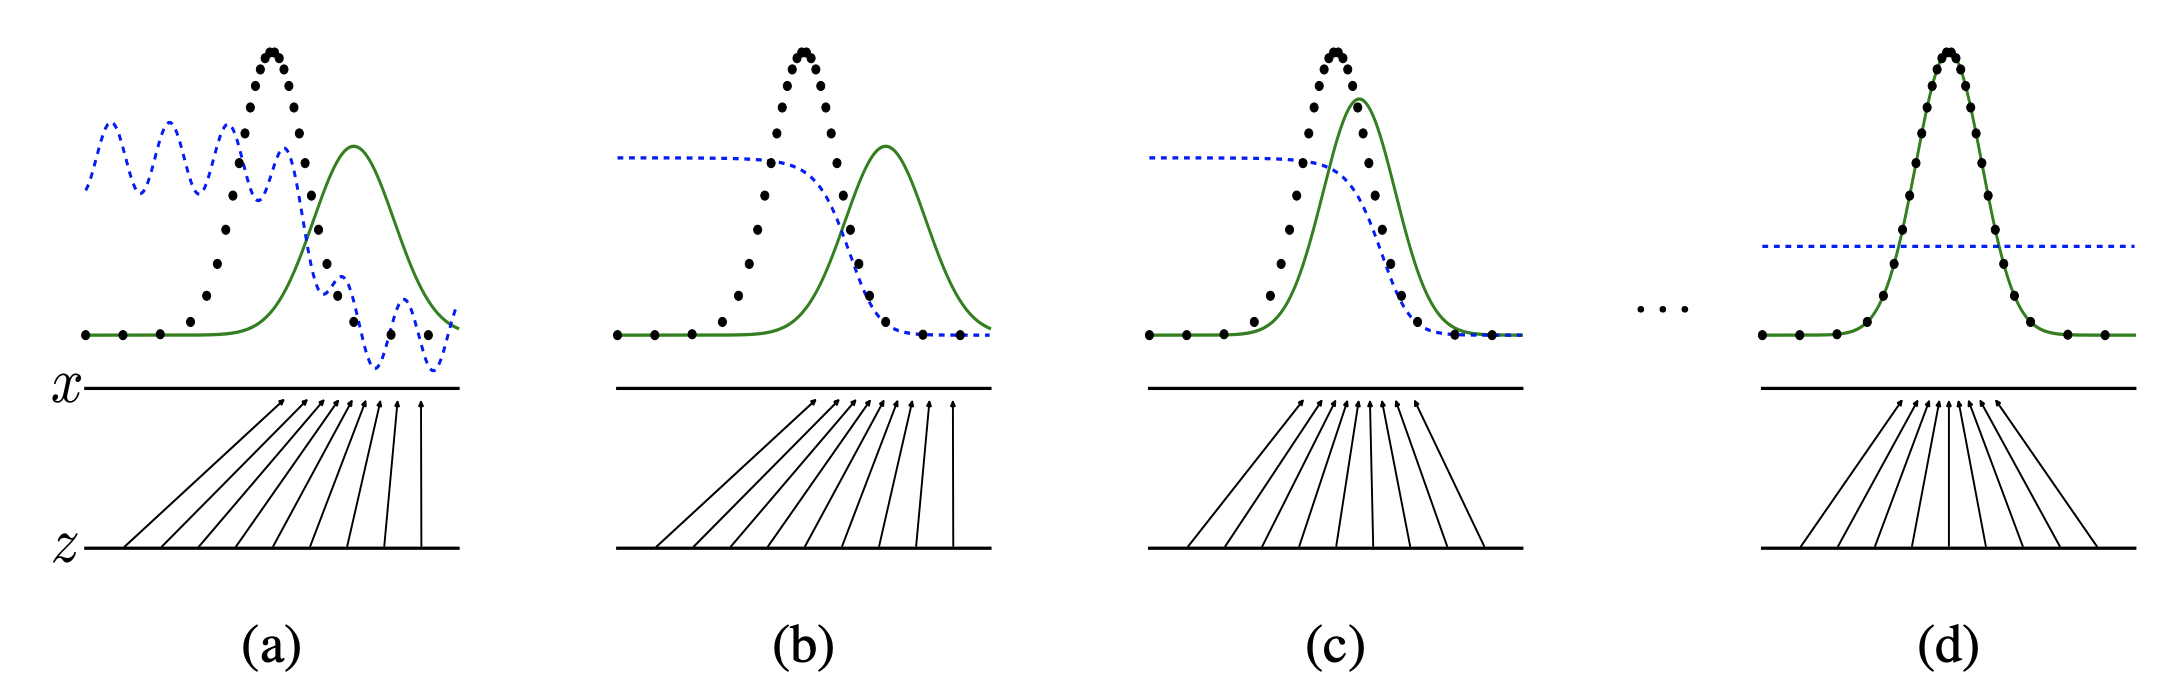
\includegraphics[width=1.0\linewidth]{figs/gan_1}
	\end{figure}
	\myfootnotewithlink{https://arxiv.org/abs/1406.2661}{Goodfellow I. J. et al. Generative Adversarial Networks, 2014}
\end{frame}
%=======
\begin{frame}{Recap of previous lecture}
	\begin{block}{Main problems of standard GAN}
		\begin{itemize}
			\item Vanishing gradients (solution: non-saturating GAN);
			\item Mode collapse (caused by Jensen-Shannon divergence).
		\end{itemize}
	\end{block}
	\begin{block}{Standard GAN}
		\vspace{-0.2cm}
		\[
		\min_{\btheta} \max_{\bphi} \left[ \bbE_{\pi(\bx)} \log D_{\bphi}(\bx) + \bbE_{p(\bz)} \log (1 - D_{\bphi}(\bG_{\btheta}(\bz))) \right]
		\]
		\vspace{-0.4cm}
	\end{block}
	\vspace{-0.1cm}
	\begin{block}{Informal theoretical results}
		The real images distribution $\pi(\bx)$ and the generated images distribution $p(\bx | \btheta)$ are low-dimensional and have disjoint supports. In this case
		\vspace{-0.3cm}
		\[
		KL(\pi || p) = KL(p || \pi) = \infty, \quad JSD(\pi || p) = \log 2.
		\]
	\end{block}
	\myfootnote{\href{https://arxiv.org/abs/1406.2661}{Goodfellow I. J. et al. Generative Adversarial Networks, 2014} \\
		\href{https://arxiv.org/abs/1701.04862}{Arjovsky M., Bottou L. Towards Principled Methods for Training Generative Adversarial Networks, 2017}}
\end{frame}
%=======
\begin{frame}{Recap of previous lecture}
	\begin{figure}
		\centering
		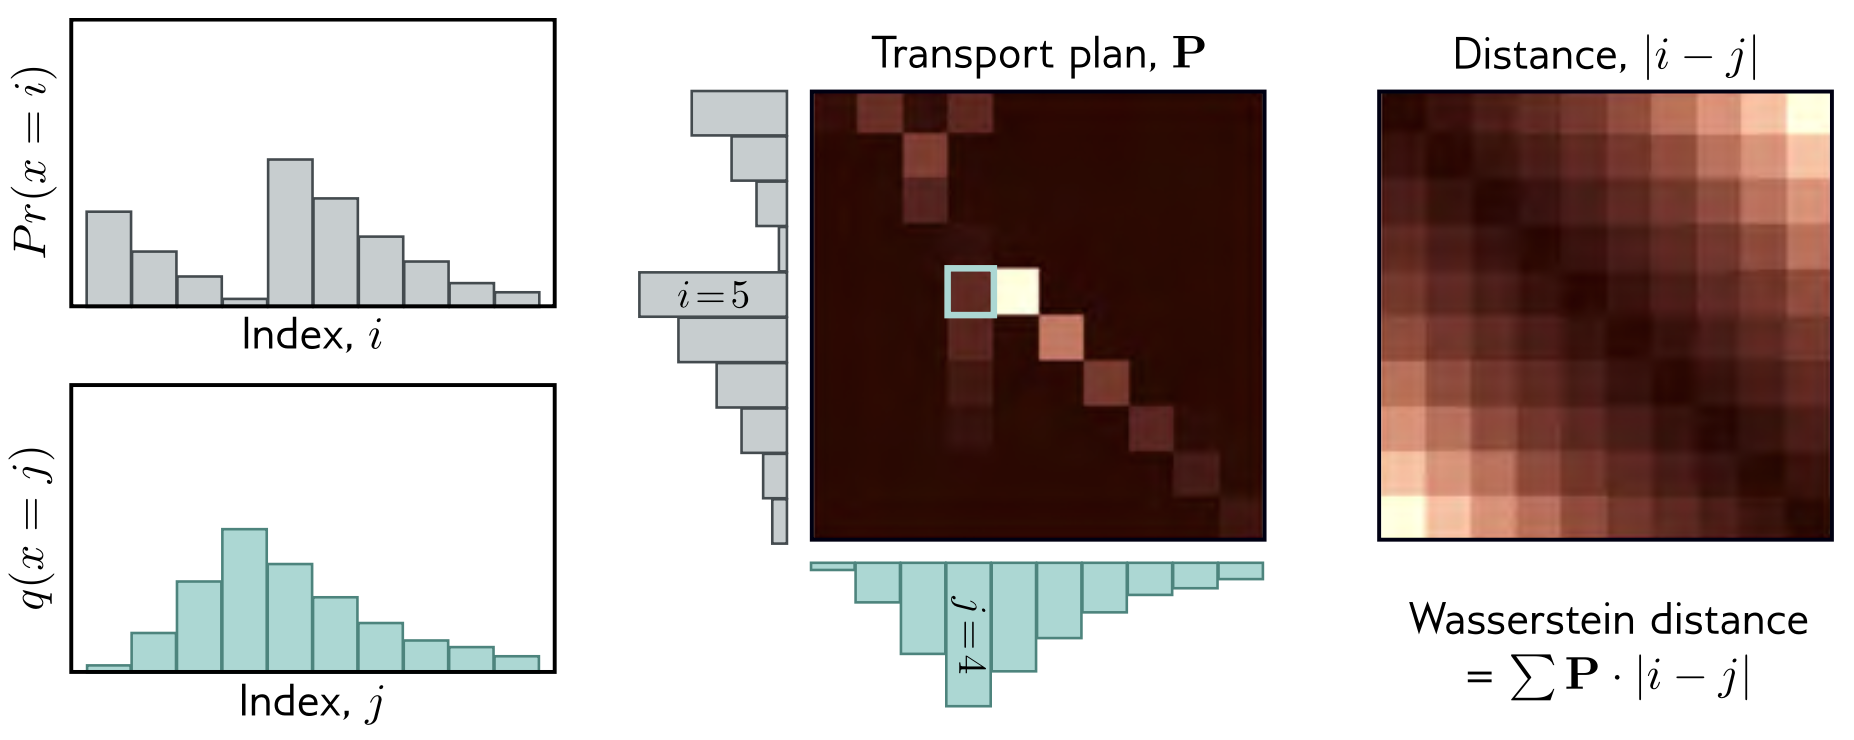
\includegraphics[width=0.8\linewidth]{figs/discrete_wasserstein}
	\end{figure}
	\vspace{-0.3cm}
	\begin{block}{Wasserstein distance}
		\vspace{-0.7cm}
		\[
		W(\pi, p) = \inf_{\gamma \in \Gamma(\pi, p)} \bbE_{(\bx, \by) \sim \gamma} \| \bx - \by \| =  \inf_{\gamma \in \Gamma(\pi, p)} \int \| \bx - \by \| \gamma (\bx, \by) d \bx d \by
		\]
		\vspace{-0.5cm}
		\begin{itemize}
			\item $\gamma(\bx, \by)$ -- transportation plan (the amount of "dirt" that should be transported from point $\bx$ to point $\by$).
			\item $\Gamma(\pi, p)$ -- the set of all joint distributions $\gamma (\bx, \by)$ with marginals $\pi$ and $p$ ($\int \gamma(\bx, \by) d \bx = p(\by)$, $\int \gamma(\bx, \by) d \by = \pi(\bx)$).
			\item $\gamma(\bx, \by)$ -- the amount, $\|\bx - \by \|$-- the distance.
		\end{itemize}
	\end{block}
	\myfootnotewithlink{https://udlbook.github.io/udlbook/}{Simon J.D. Prince. Understanding Deep Learning, 2023}
\end{frame}
%=======
\begin{frame}{Outline}
	\tableofcontents
\end{frame}
%=======
\section{Wasserstein GAN}
%=======
\begin{frame}{Wasserstein GAN}
	\begin{block}{Wasserstein distance}
		\vspace{-0.5cm}
		\[
		W(\pi || p) = \inf_{\gamma \in \Gamma(\pi, p)} \bbE_{(\bx, \by) \sim \gamma} \| \bx - \by \| =  \inf_{\gamma \in \Gamma(\pi, p)} \int \| \bx - \by \| \gamma (\bx, \by) d \bx d \by
		\]
		\vspace{-0.3cm}
	\end{block}
	The infimum across all possible joint distributions in $\Gamma(\pi, p)$ is intractable.
	\begin{block}{Theorem (Kantorovich-Rubinstein duality)}
		\vspace{-0.3cm}
		\[
		W(\pi || p) = \frac{1}{K} \max_{\| f \|_L \leq K} \left[ \bbE_{\pi(\bx)} f(\bx)  - \bbE_{p(\bx)} f(\bx)\right],
		\]
		where $f : \bbR^m \rightarrow \bbR$, $\| f \|_L \leq K$ are $K-$Lipschitz continuous functions ($f: \cX \rightarrow \bbR$)
		\vspace{-0.2cm}
		\[
		|f(\bx_1) - f(\bx_2)| \leq K \| \bx_1 - \bx_2 \|, \quad \text{for all } \bx_1, \bx_2 \in \cX.
		\]
		\vspace{-0.6cm}
	\end{block}
	Now we need only samples to get Monte Carlo estimate for $W(\pi || p)$.
	
	\myfootnotewithlink{https://arxiv.org/abs/1701.07875}{Arjovsky M., Chintala S., Bottou L. Wasserstein GAN, 2017}
\end{frame}
%=======
\begin{frame}{Wasserstein GAN}
	\begin{block}{Theorem (Kantorovich-Rubinstein duality)}
		\[
		W(\pi || p) = \frac{1}{K} \max_{\| f \|_L \leq K} \left[ \bbE_{\pi(\bx)} f(\bx)  - \bbE_{p(\bx)} f(\bx)\right],
		\]
	\end{block}
	\begin{itemize}
		\item Now we have to ensure that $f$ is $K$-Lipschitz continuous.
		\item Let $f_{\bphi}(\bx)$ be a feedforward neural network parametrized by~$\bphi$.
		\item If parameters $\bphi$ lie in a compact set $\boldsymbol{\Phi}$ then $f_{\bphi}(\bx)$ will be $K$-Lipschitz continuous function. 
		\item Let the parameters be clamped to a fixed box $\boldsymbol{\Phi} \in [-c, c]^d$ (e.x. $c = 0.01$) after each gradient update.
	\end{itemize}
	\begin{multline*}
		K \cdot W(\pi || p) = \max_{\| f \|_L \leq K} \left[ \bbE_{\pi(\bx)} f(\bx)  - \bbE_{p(\bx)} f(\bx)\right] \geq \\  \geq \max_{\bphi \in \boldsymbol{\Phi}} \left[ \bbE_{\pi(\bx)} f_{\bphi}(\bx)  - \bbE_{p(\bx)} f_{\bphi}(\bx)\right]
	\end{multline*}
	
	\myfootnotewithlink{https://arxiv.org/abs/1701.07875}{Arjovsky M., Chintala S., Bottou L. Wasserstein GAN, 2017}
\end{frame}
%=======
\begin{frame}{Wasserstein GAN}
	\begin{block}{Standard GAN objective}
		\vspace{-0.2cm}
		\[
		\min_{\btheta} \max_{\bphi} \bbE_{\pi(\bx)} \log D_{\bphi}(\bx) + \bbE_{p(\bz)} \log (1 - D_{\bphi}(\bG_{\btheta}(\bz)))
		\]
		\vspace{-0.3cm}
	\end{block}
	\begin{block}{WGAN objective}
		\vspace{-0.3cm}
		\[
		\min_{\btheta} {\color{violet}W(\pi || p)} \approx \min_{\btheta} {\color{violet}\max_{\bphi \in \boldsymbol{\Phi}} \left[ \bbE_{\pi(\bx)} f_{\bphi}(\bx)  - \bbE_{p(\bz)} f_{\bphi}(\bG_{\btheta}(\bz))\right]}.
		\]
		\vspace{-0.3cm}
	\end{block}
	\begin{itemize}
		\item Discriminator $D$ is similar to the function $f$, but it is not a classifier anymore. In the WGAN model, function~$f$ is usually called $\textbf{critic}$.
		\item \textit{"Weight clipping is a clearly terrible way to enforce a Lipschitz constraint"}. 
		\begin{itemize}
			\item If the clipping parameter $c$ is too large, it is hard to train the critic till optimality.
			\item If the clipping parameter $c$ is too small, it could lead to vanishing gradients.
		\end{itemize}
	\end{itemize}
	
	\myfootnotewithlink{https://arxiv.org/abs/1701.07875}{Arjovsky M., Chintala S., Bottou L. Wasserstein GAN, 2017}
\end{frame}
%=======
\begin{frame}{Wasserstein GAN}
	\begin{minipage}[t]{0.6\columnwidth}
		\begin{itemize}
			\item WGAN has non-zero gradients for disjoint supports.
			\item $JSD(\pi || p)$ correlates poorly with the sample quality. Stays constast nearly maximum value $\log 2 \approx 0.69$.
			\item $W(\pi || p)$ is highly correlated with the sample quality. 
		\end{itemize}
	\end{minipage}%
	\begin{minipage}[t]{0.4\columnwidth}
		\begin{figure}
			\centering
			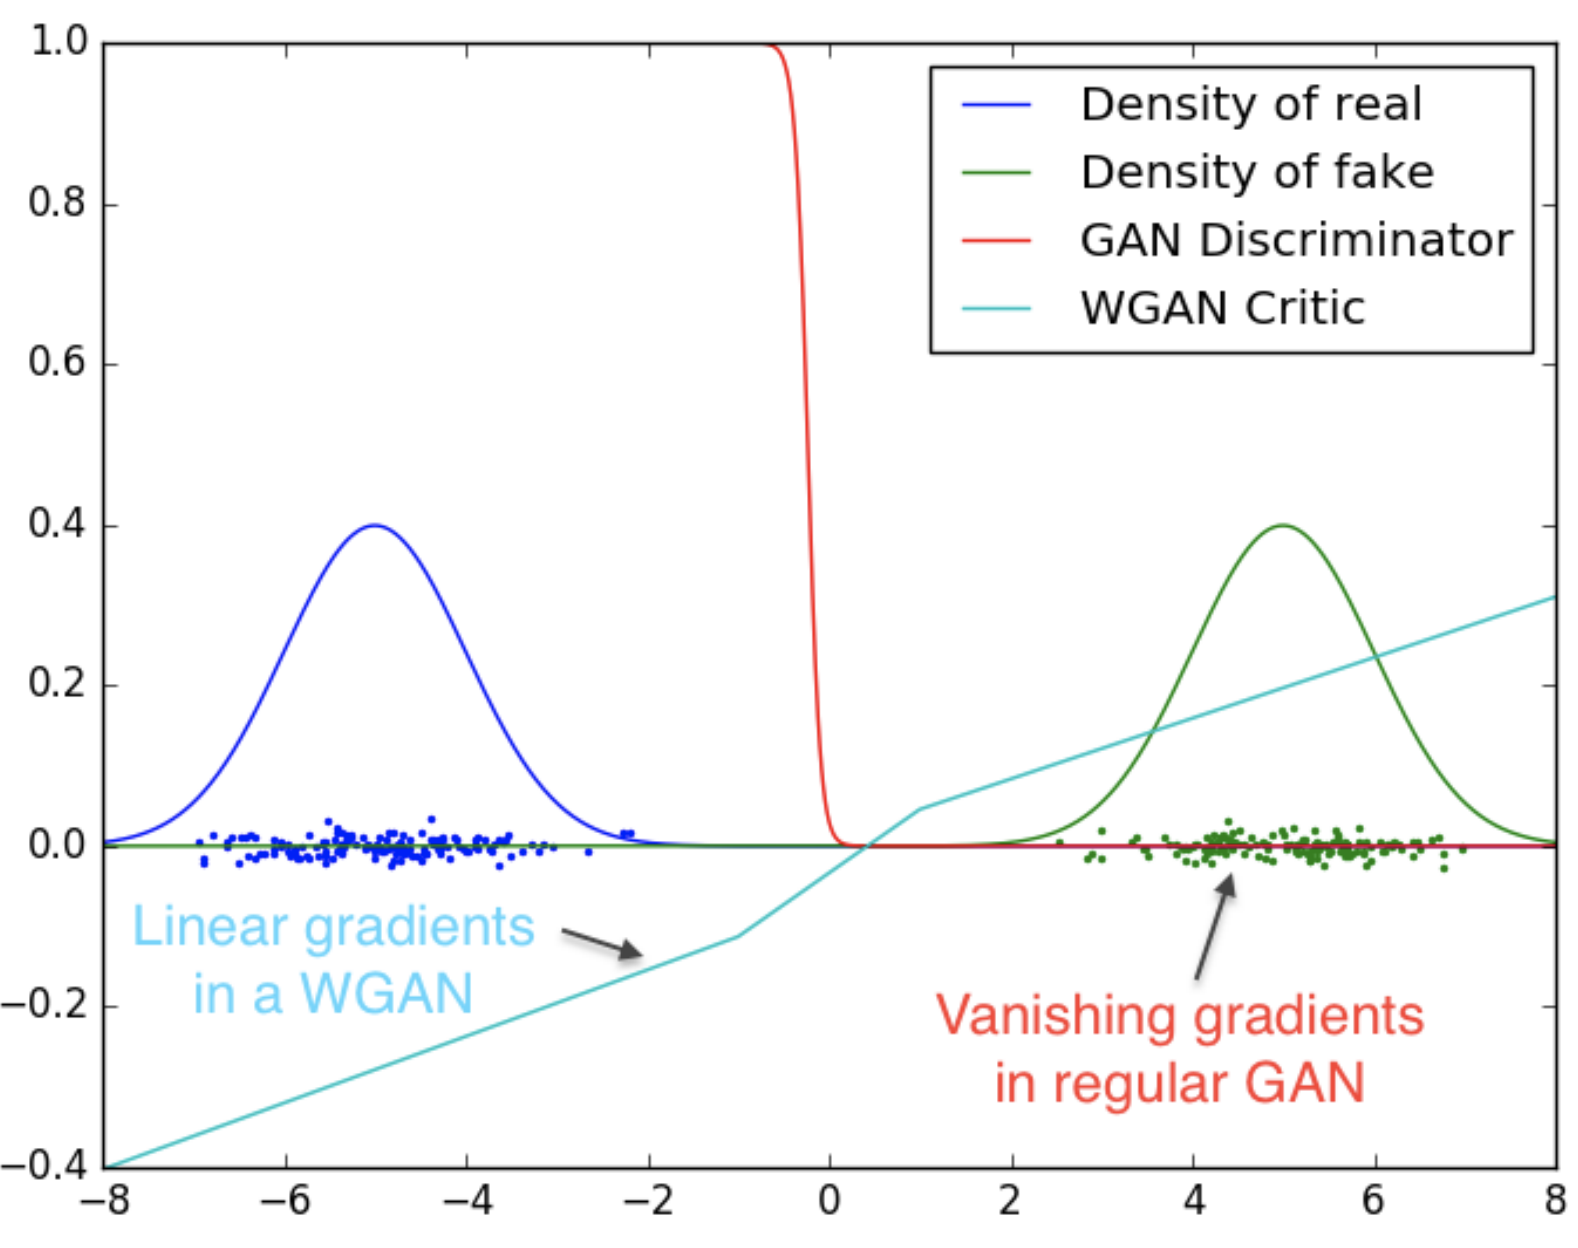
\includegraphics[width=\linewidth]{figs/wgan_toy}
		\end{figure}
	\end{minipage}
	\begin{minipage}[t]{0.5\columnwidth}
		\begin{figure}
			\centering
			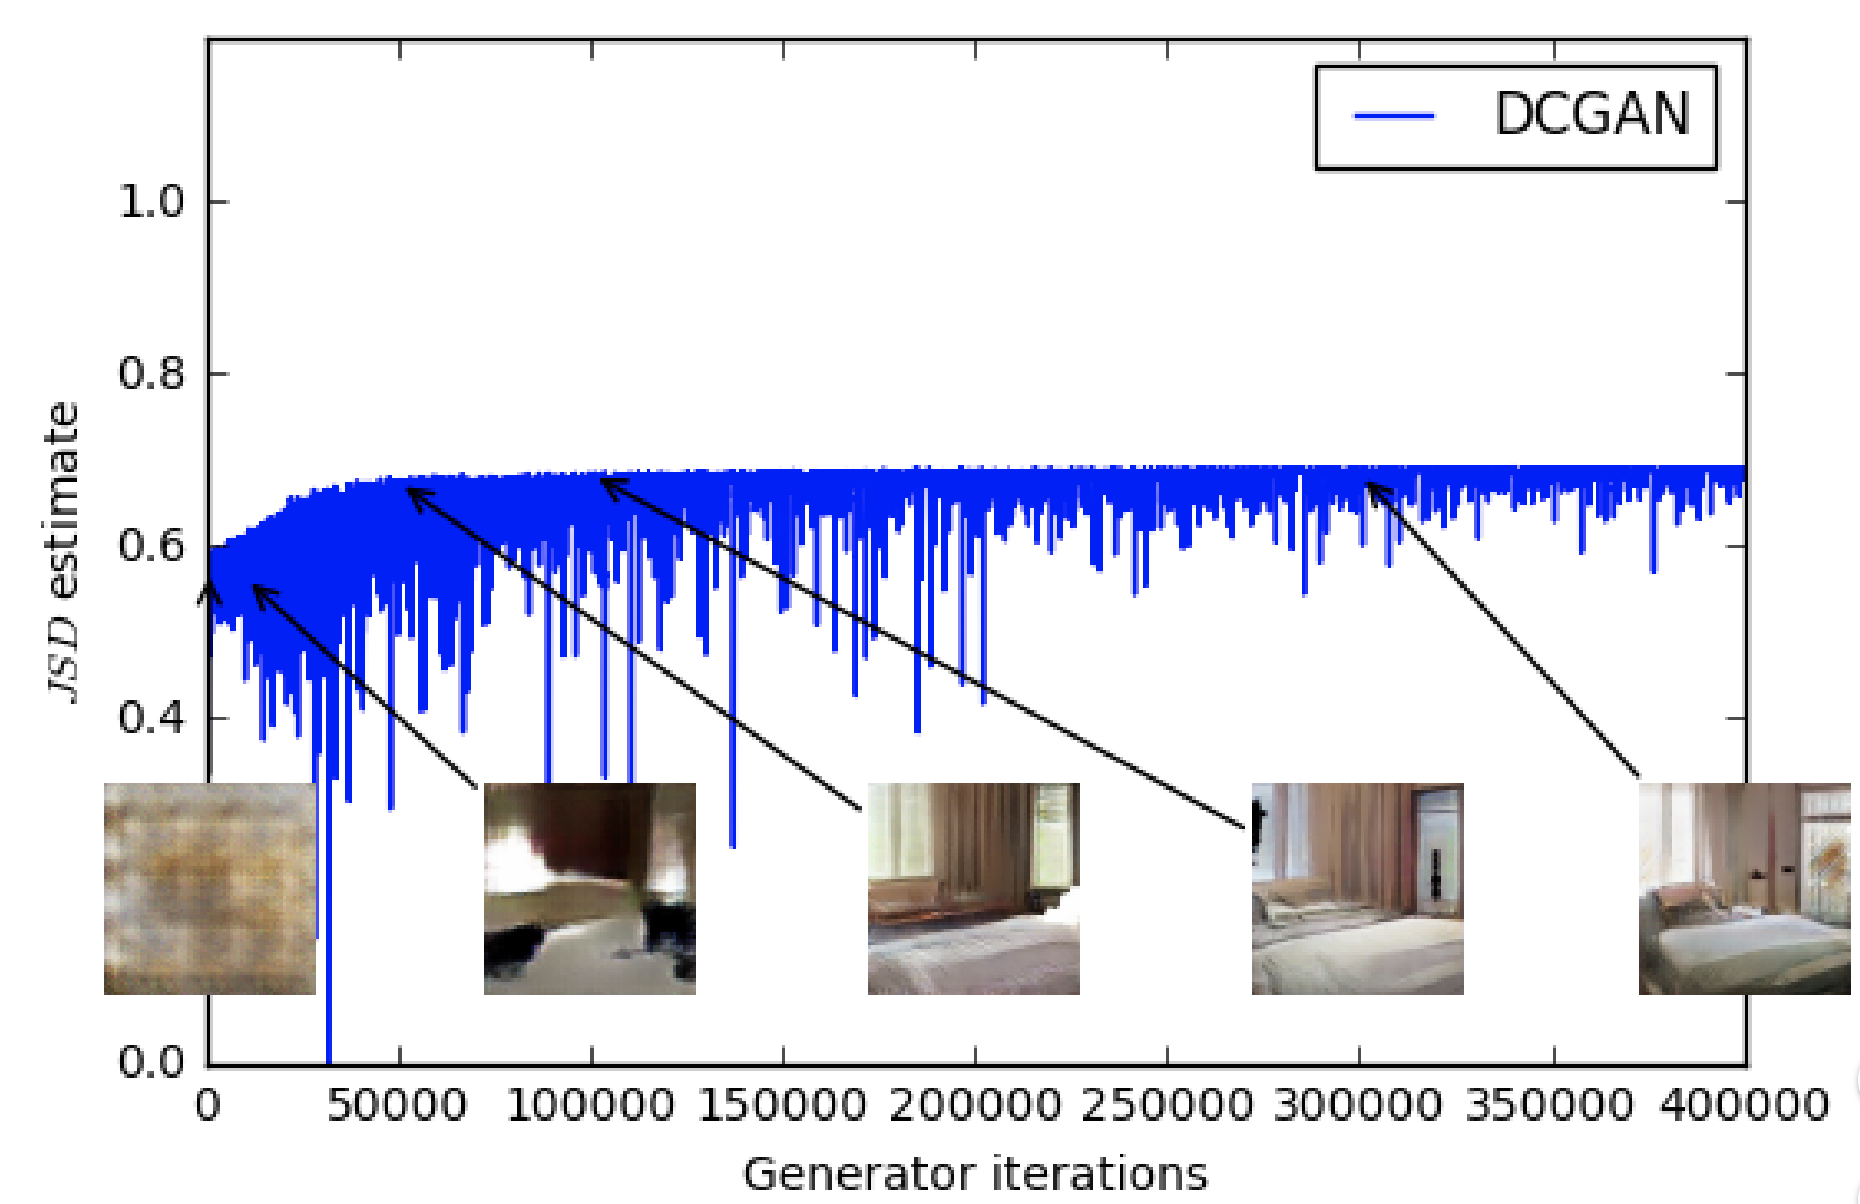
\includegraphics[width=1.0\linewidth]{figs/dcgan_quality}
		\end{figure}
	\end{minipage}%
	\begin{minipage}[t]{0.5\columnwidth}
		\begin{figure}
			\centering
			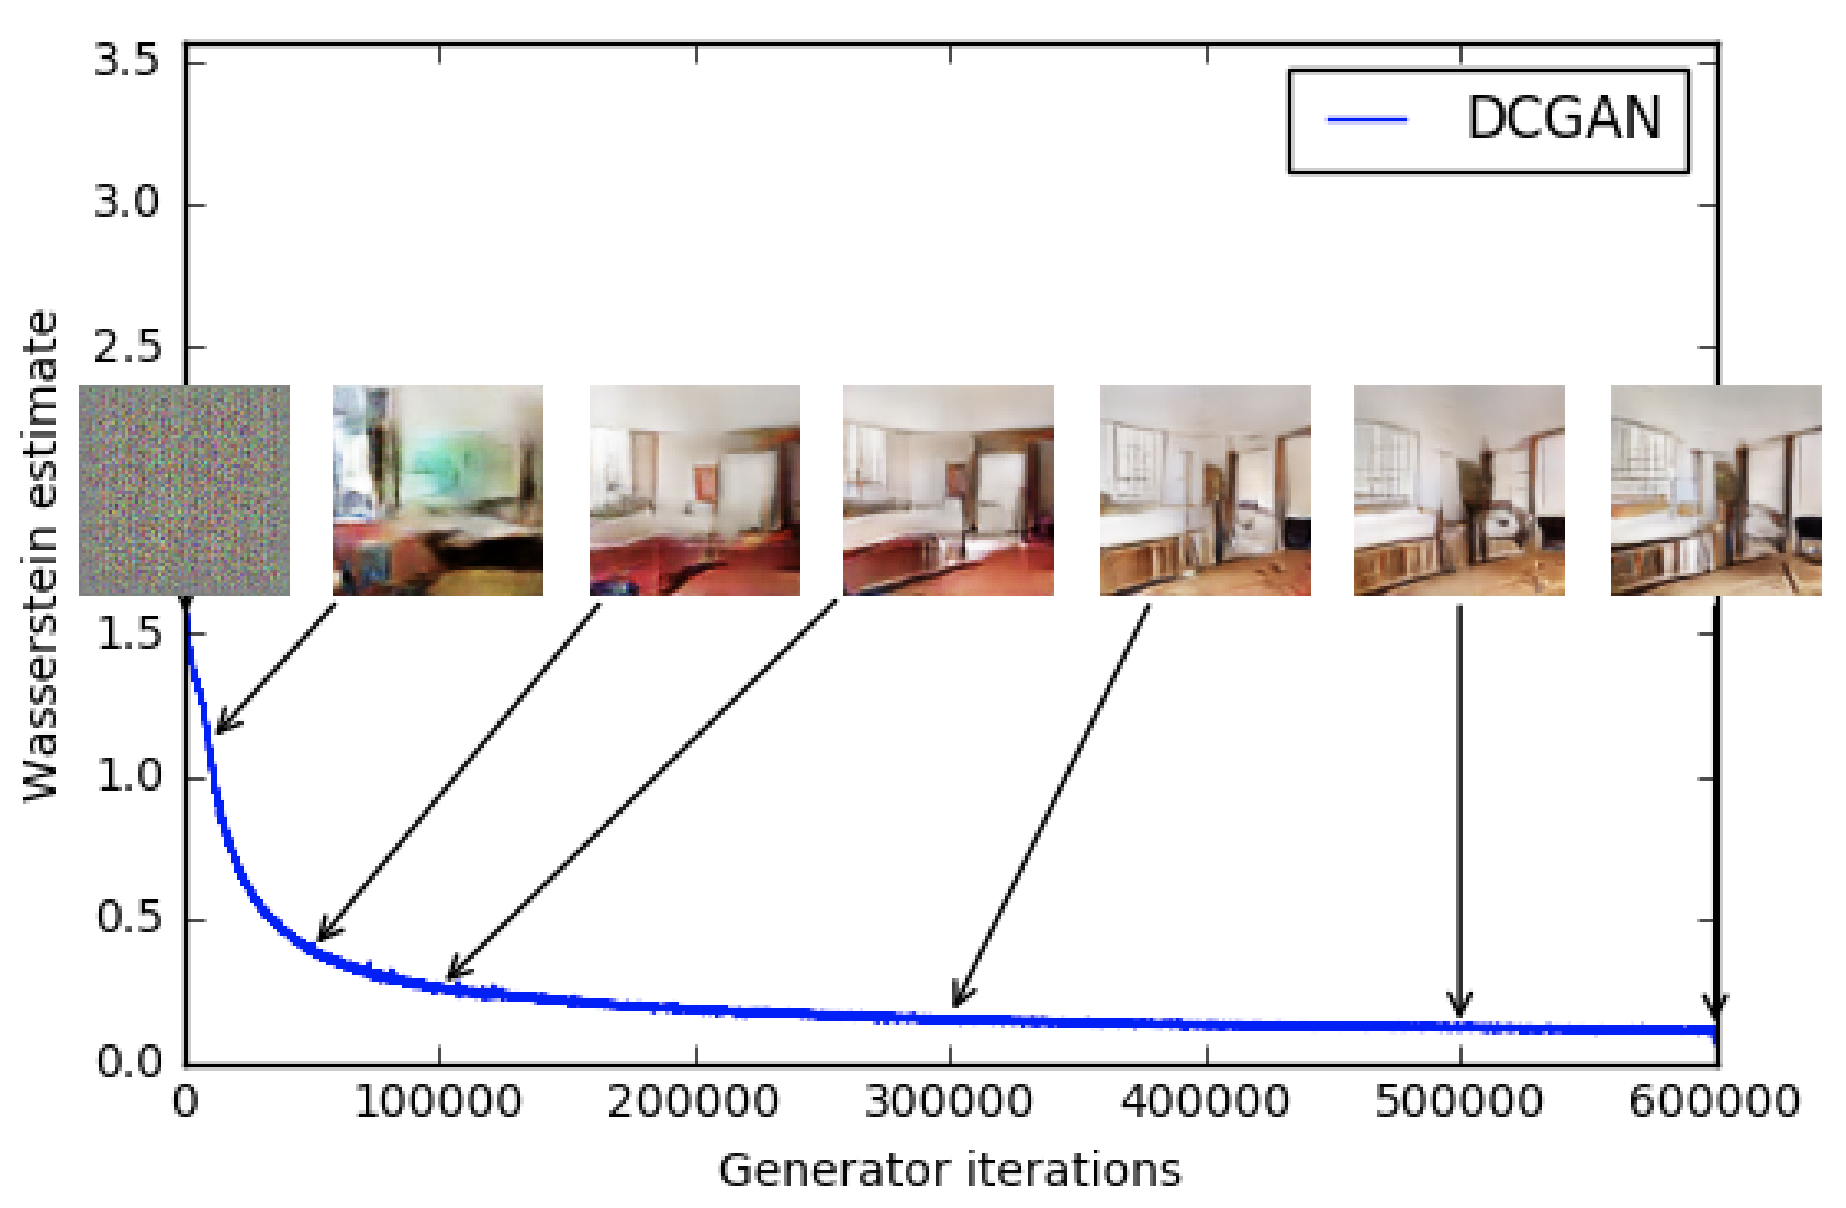
\includegraphics[width=1.0\linewidth]{figs/wgan_quality}
		\end{figure}
	\end{minipage}
	
	\myfootnotewithlink{https://arxiv.org/abs/1701.07875}{Arjovsky M., Chintala S., Bottou L. Wasserstein GAN, 2017}
\end{frame}
%=======
\section{f-divergence minimization}
%=======
\begin{frame}{Divergences}
	\begin{itemize}
		\item Forward KL divergence in the maximum likelihood estimation.
		\item Reverse KL in the variational inference (KL term in ELBO).
		\item JS divergence in the standard GAN.
		\item Wasserstein distance in WGAN.
	\end{itemize}
	\begin{block}{What is a divergence?}
		Let $\cP$ be the set of all possible probability distributions. Then $D: \cP \times \cP \rightarrow \bbR$ is a divergence if 
		\begin{itemize}
			\item $D(\pi || p) \geq 0$ for all $\pi, p \in \cP$;
			\item $D(\pi || p) = 0$ if and only if $\pi \equiv p$.
		\end{itemize}
	\end{block}
	\begin{block}{General divergence minimization task}
		\vspace{-0.3cm}
		\[
			\min_p D(\pi || p)
		\]
		\vspace{-0.7cm}
	\end{block}
	\begin{block}{Chalenge}
		We do not know the real distribution $\pi(\bx)$!
	\end{block}
\end{frame}
%=======
\begin{frame}{f-divergence family}
	
	\begin{block}{f-divergence}
		\vspace{-0.3cm}
		\[
		D_f(\pi || p) = \bbE_{p(\bx)}  f\left( \frac{\pi(\bx)}{p(\bx)} \right)  = \int p(\bx) f\left( \frac{\pi(\bx)}{p(\bx)} \right) d \bx.
		\]
		Here $f: \bbR_+ \rightarrow \bbR$ is a convex, lower semicontinuous function satisfying $f(1) = 0$.
	\end{block}
	\begin{figure}
		\centering
		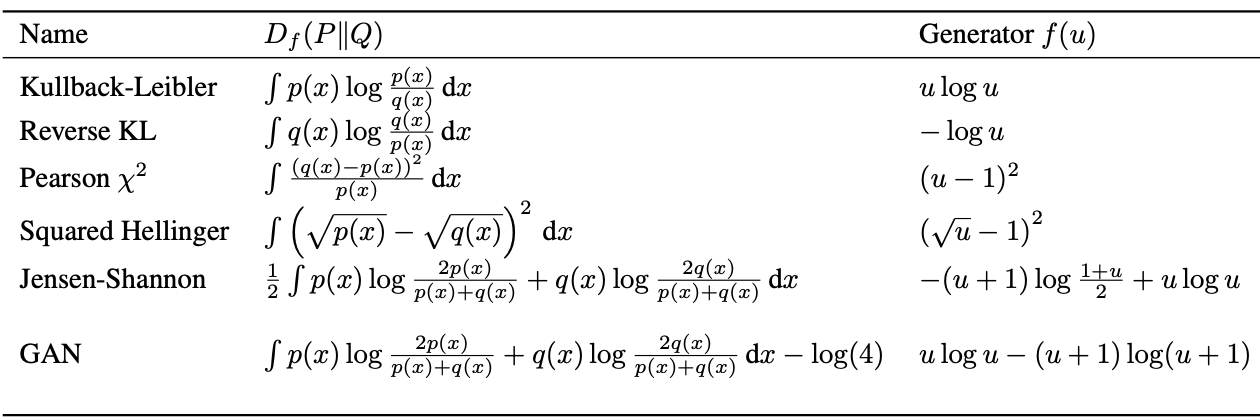
\includegraphics[width=\linewidth]{figs/f_divs}
	\end{figure}
	\myfootnotewithlink{https://arxiv.org/abs/1606.00709}{Nowozin S., Cseke B., Tomioka R. f-GAN: Training Generative Neural Samplers using Variational Divergence Minimization, 2016}
\end{frame}
%=======
\begin{frame}{f-divergence family}
	\vspace{-0.3cm}
	\begin{block}{Fenchel conjugate}
		\vspace{-0.5cm}
		\[
		f^*(t) = \sup_{u \in \text{dom}_f} \left( ut - f(u) \right), \quad f(u) = \sup_{t \in \text{dom}_{f^*}} \left( ut - f^*(t) \right)
		\]
		\vspace{-0.3cm}
	\end{block}
	\vspace{-0.3cm}
	\begin{minipage}[t]{0.5\columnwidth}
		\begin{figure}
			\centering
			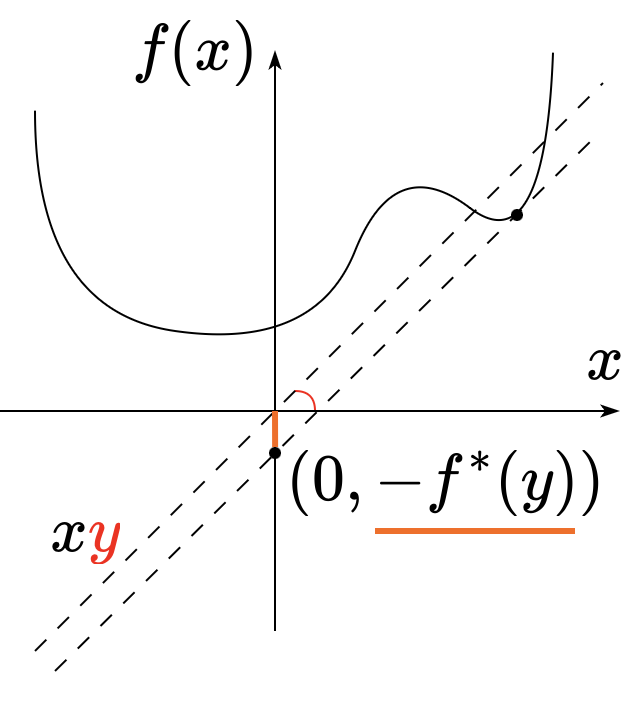
\includegraphics[width=0.8\linewidth]{figs/conj}
		\end{figure}
	\end{minipage}%
	\begin{minipage}[t]{0.5\columnwidth}
		\begin{figure}
			\centering
			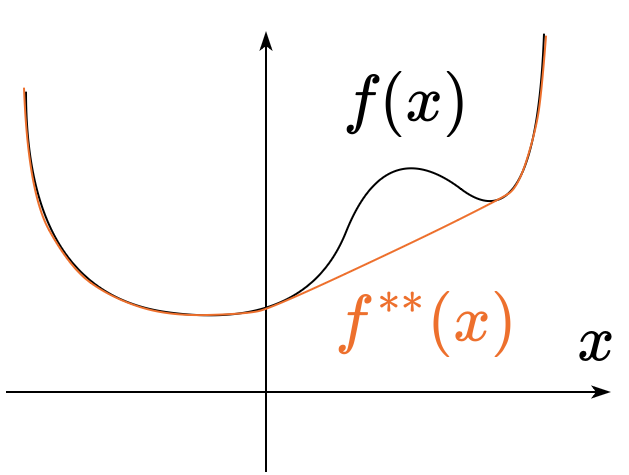
\includegraphics[width=0.85\linewidth]{figs/double_conj}
		\end{figure}
	\end{minipage}
	\textbf{Important property:} $ f^{**} = f$ for convex $f$.
	\myfootnotewithlink{https://fmin.xyz/docs/theory/Conjugate\%20function.html}{image credit: https://fmin.xyz/docs/theory/Conjugate\%20function.html}
\end{frame}
%=======
\begin{frame}{f-divergence family}
	\vspace{-0.3cm}
	\[
		f^*(t) = \sup_{u \in \text{dom}_f} \left( ut - f(u) \right), \quad f(u) = \sup_{t \in \text{dom}_{f^*}} \left( ut - f^*(t) \right)
	\]
	\vspace{-0.5cm}
	\begin{block}{Variational f-divergence estimation}
		\vspace{-0.7cm}
		\begin{multline*}
			D_f(\pi || p) = \bbE_{p(\bx)}  f\left( \frac{\pi(\bx)}{p(\bx)} \right)  = \int p(\bx) {\color{violet}f\left( \frac{\pi(\bx)}{p(\bx)} \right) } d \bx = \\ = \int p(\bx) {\color{violet} \sup_{t \in \text{dom}_{f^*}} \left( \frac{\pi(\bx)}{p(\bx)} t - f^*(t) \right)} d \bx = \\ 
			= {\color{olive}\int} {\color{teal} \sup_{t \in \text{dom}_{f^*}}} \left( \pi(\bx)t - p(\bx) f^*(t) \right) d \bx \geq \\
		 \geq {\color{teal}\sup_{T \in \cT}} {\color{olive}\int} \left( \pi(\bx)T(\bx) - p(\bx) f^*(T(\bx)) \right) d \bx = \\
		 = \sup_{T \in \cT} \left[\bbE_{\pi}T(\bx) -  \bbE_p f^*(T(\bx)) \right]
		\end{multline*}
		\vspace{-0.6cm}
	\end{block}
	\myfootnotewithlink{https://arxiv.org/abs/1606.00709}{Nowozin S., Cseke B., Tomioka R. f-GAN: Training Generative Neural Samplers using Variational Divergence Minimization, 2016}
\end{frame}
%=======
\begin{frame}{f-divergence family}
	\begin{block}{Variational divergence estimation}
		\vspace{-0.2cm}
		\[
			D_f(\pi || p) \geq \sup_{T \in \cT} \left[\bbE_{\pi}T(\bx) -  \bbE_p f^*(T(\bx)) \right]
		\]
		\vspace{-0.3cm}
		\begin{itemize}
			\item Here $\cT$ is a predefined class of functions.
			\item The lower bound is tight for $T^*(\bx) = f'\left( \frac{\pi(\bx)}{p(\bx)} \right)$. 
		\end{itemize}
		\vspace{-0.3cm}
	\end{block}
	\begin{block}{Example (JSD)}
		\begin{itemize}
			\item Let define function $f$ and its conjugate $f^*$
			\[ 
				f(u) = u \log u - (u + 1) \log (u + 1), \quad f^*(t) = - \log (1 - e^t).
			\]
			\item Let reparametrize $T(\bx) = \log D(\bx)$ ($D(\bx) \in [0, 1]$).
		\end{itemize}
		\vspace{-0.4cm}
	\end{block}
	\[
		\min_{G} \max_D \left[ \bbE_{\pi(\bx)} \log D(\bx) + \bbE_{p(\bz)} \log (1 - D(\bG(\bz))) \right]
	\]

	\myfootnotewithlink{https://arxiv.org/abs/1606.00709}{Nowozin S., Cseke B., Tomioka R. f-GAN: Training Generative Neural Samplers using Variational Divergence Minimization, 2016}
\end{frame}
%=======
\begin{frame}{f-divergence family}
	\begin{block}{Variational divergence estimation}
		\[
			D_f(\pi || p) \geq \sup_{T \in \cT} \left[\bbE_{\pi}T(\bx) -  \bbE_p f^*(T(\bx)) \right]
		\]
		\vspace{-0.3cm}
	\end{block}
	\textbf{Note:} To evaluate the lower bound we only need samples from $\pi(\bx)$ and $p(\bx)$. Hence, we are able to fit the implicit generative model.
	\begin{figure}
		\centering
		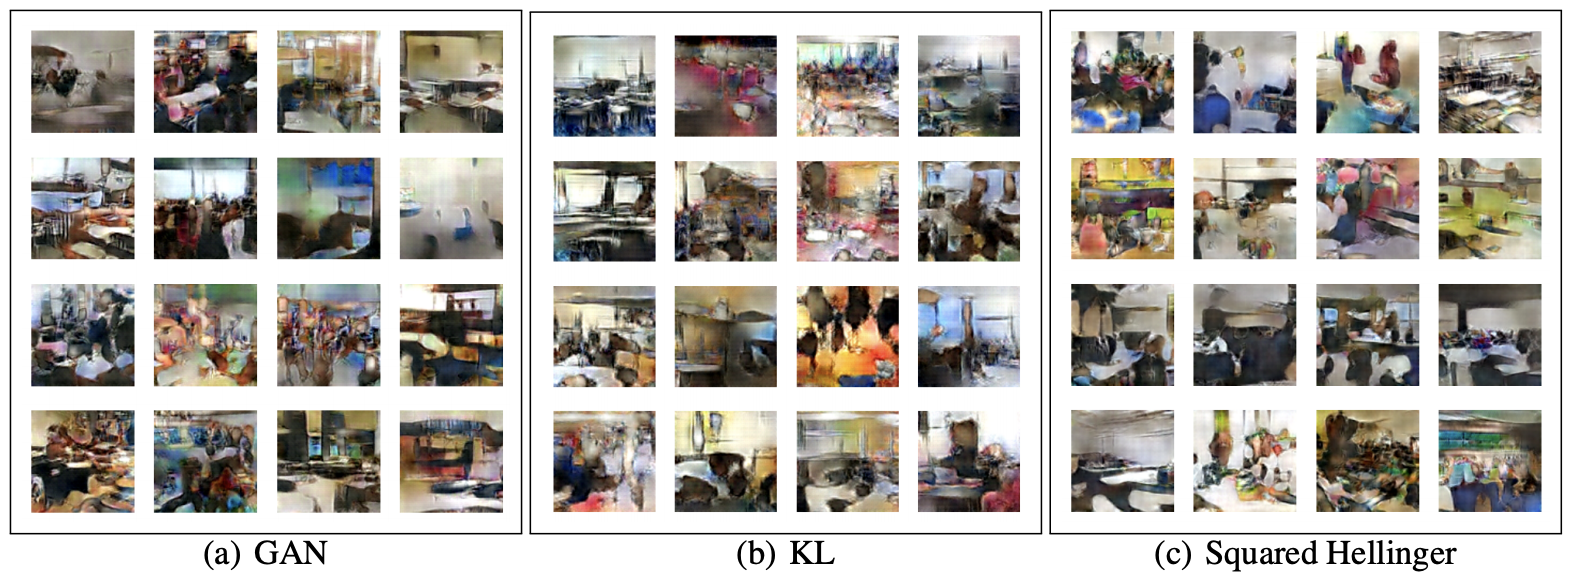
\includegraphics[width=1.0\linewidth]{figs/f_div_results}
	\end{figure}

	\myfootnotewithlink{https://arxiv.org/abs/1606.00709}{Nowozin S., Cseke B., Tomioka R. f-GAN: Training Generative Neural Samplers using Variational Divergence Minimization, 2016}
\end{frame}
%=======
\section{Evaluation of likelihood-free models}
%=======
\begin{frame}{Evaluation of likelihood-free models}
	\begin{block}{Likelihood-based models}
		\begin{itemize}
			\item \textbf{train part:} fit the model.
			\item \textbf{validation part:} tune the hyperparameters.
			\item \textbf{test part:} evaluate generalization by reporting the likelihood.
		\end{itemize}
	\end{block}
	Not all models have tractable likelihood \\ (VAE: compare ELBO values; GAN: \textbf{???}).
	\begin{block}{What do we want from samples?}
		\begin{itemize}
			\item Sharpness
			\begin{figure}
				\centering
				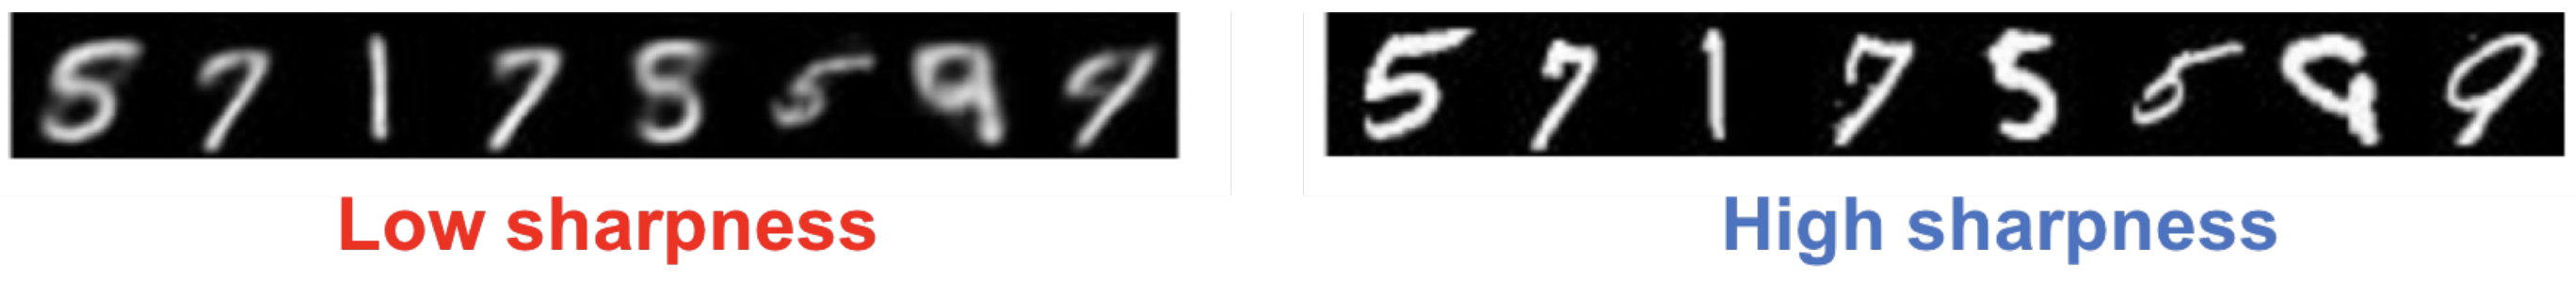
\includegraphics[width=0.9\linewidth]{figs/sharpness}
			\end{figure}
			\item Diversity
			\begin{figure}
				\centering
				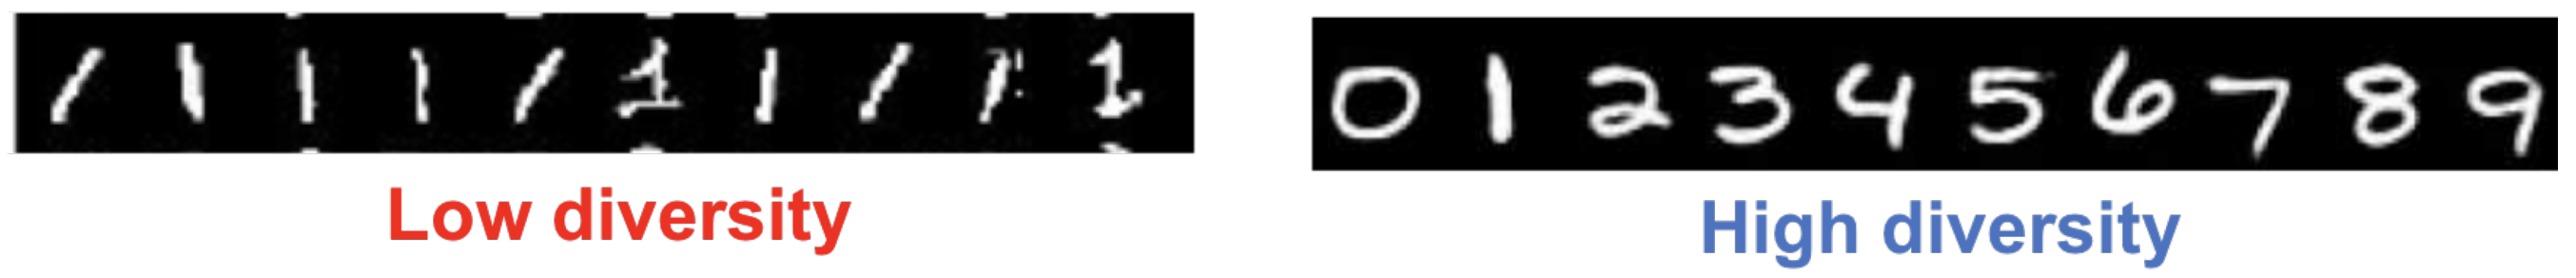
\includegraphics[width=0.9\linewidth]{figs/diversity}
			\end{figure}
		\end{itemize}
	\end{block}
	\myfootnotewithlink{https://deepgenerativemodels.github.io}{image credit: https://deepgenerativemodels.github.io}
\end{frame}
%=======
\begin{frame}{Evaluation of likelihood-free models}
	Let take some pretrained image classification model to get the conditional label distribution $p(y | \bx)$ (e.g. ImageNet classifier).
	\begin{block}{What do we want from samples?}
		\begin{itemize}
			\item \textbf{Sharpness.}
			The \textbf{conditional} distribution $p(y | \bx)$ should have low entropy (each image $\bx$ depicts distinctly recognizable object).
			\item \textbf{Diversity.}
			The \textbf{marginal} distribution $p(y) = \int p(y | \bx) p(\bx) d \bx$ should have high entropy (we generate all classes uniformly).
		\end{itemize}
	\end{block}
	\vspace{-0.3cm}
	\begin{figure}
		\centering
		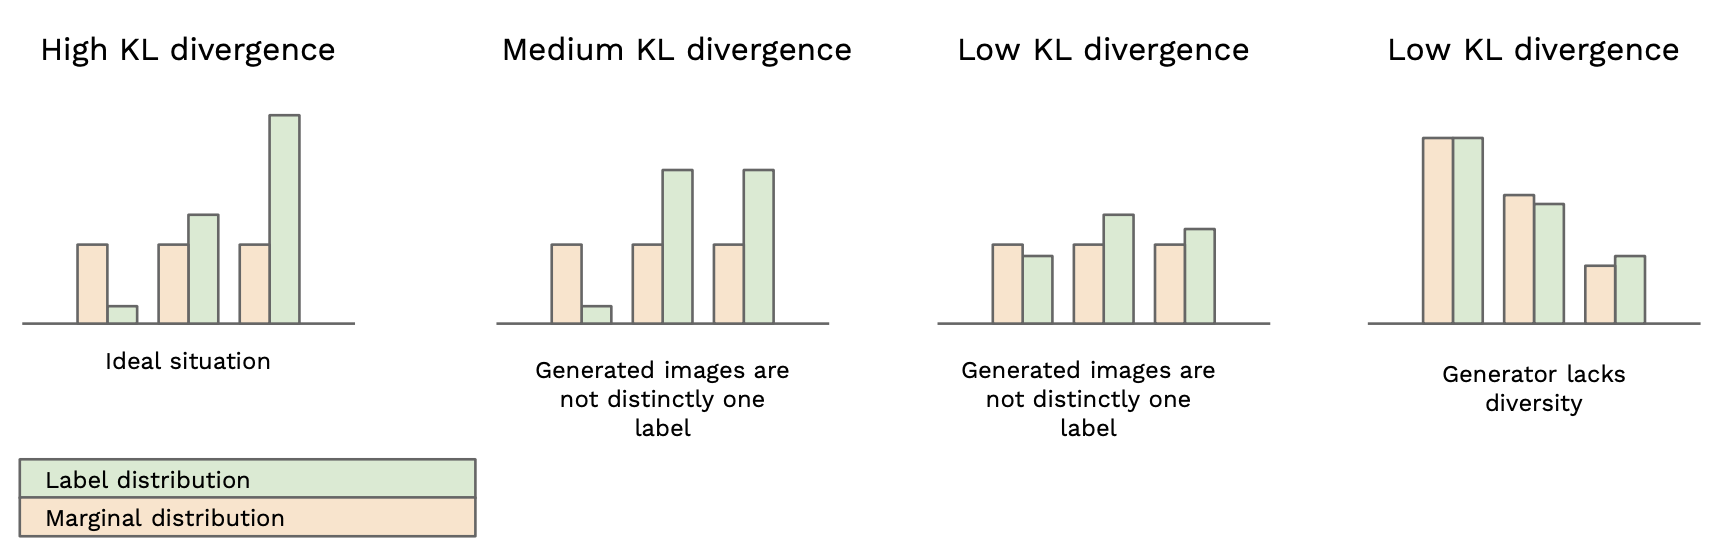
\includegraphics[width=1.0\linewidth]{figs/is_toy}
	\end{figure}
	\myfootnotewithlink{https://medium.com/octavian-ai/a-simple-explanation-of-the-inception-score-372dff6a8c7a}{image credit: https://medium.com/octavian-ai/a-simple-explanation-of-the-inception-score-372dff6a8c7a}
\end{frame}
%=======
\subsection{Frechet Inception Distance (FID)}
%=======
\begin{frame}{Frechet Inception Distance (FID)}
	\begin{block}{Wasserstein metric}
		\vspace{-0.2cm}
		\[
		W_s(\pi, p) = \inf_{\gamma \in \Gamma(\pi, p)} \left(\bbE_{(\bx, \by) \sim \gamma} \| \bx - \by \|^s\right)^{1/s}
		\]
		\vspace{-0.6cm}
	\end{block}
	\begin{block}{Theorem}
		If $\pi(\bx) = \cN(\bmu_\pi, \bSigma_\pi)$, $p(\by) = \cN(\bmu_p, \bSigma_p)$, then
		\vspace{-0.3cm}
		\[
		W_2^2(\pi, p) = \| \bmu_{\pi} - \bmu_{p}\|^2 + \text{tr} \left[ \bSigma_{\pi} + \bSigma_p - 2 \left(\bSigma_{\pi}^{1/2} \bSigma_p \bSigma_{\pi}^{1/2} \right)^{1/2} \right]
		\]
		\vspace{-0.7cm}
	\end{block}
	\begin{block}{Frechet Inception Distance}
		\vspace{-0.3cm}
		\[
			\text{FID} (\pi, p) =  W_2^2(\pi, p)
		\]
		\vspace{-0.6cm}
	\end{block}
	\begin{itemize}
		\item Representations are the outputs of the intermediate layer from the pretrained classification model.
		\item $\bmu_{\pi}$, $\bSigma_{\pi}$ and $\bmu_{p}$, $\bSigma_p$ are the statistics of the feature representations for the samples from $\pi(\bx)$ and $p(\bx | \btheta)$.
	\end{itemize}
	\myfootnotewithlink{https://arxiv.org/abs/1706.08500}{Heusel M. et al. GANs Trained by a Two Time-Scale Update Rule Converge to a Local Nash Equilibrium, 2017}
\end{frame}
%=======
\begin{frame}{Frechet Inception Distance (FID)}
	\vspace{-0.4cm}
	\[
	\text{FID} (\pi, p) =  \| \bmu_{\pi} - \bmu_{p}\|^2 + \text{tr} \left[ \bSigma_{\pi} + \bSigma_p - 2 \left(\bSigma_{\pi}^{1/2} \bSigma_p \bSigma_{\pi}^{1/2} \right)^{1/2} \right]
	\]
	\vspace{-0.3cm}
	\begin{itemize}
		\item Needs a large sample size for evaluation.
		\item Calculation of FID is slow.
		\item High dependence on the pretrained classification model.
		\item Uses the normality assumption!
	\end{itemize}
	\begin{block}{$FID(p(\bx), \cN(0, \bI))$}
		\begin{figure}
			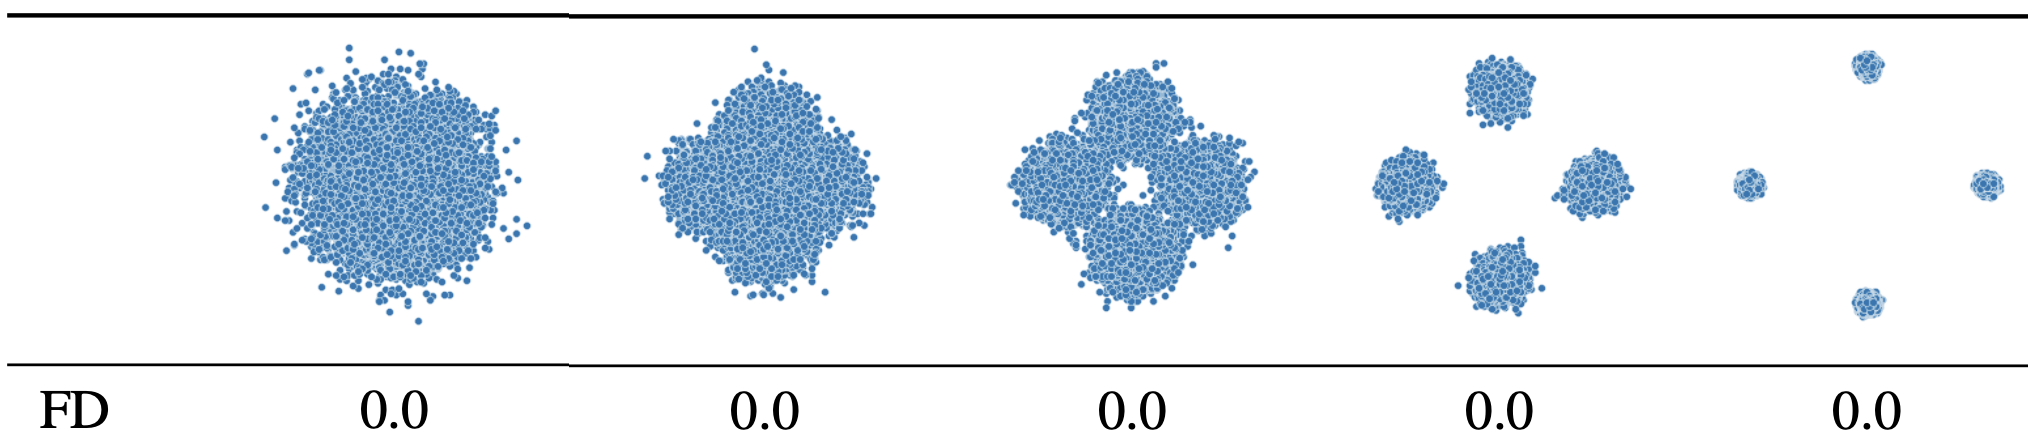
\includegraphics[width=0.95\linewidth]{figs/fid_normal}
		\end{figure}
	\end{block}

	\myfootnotewithlink{https://arxiv.org/abs/2401.09603}{Jayasumana S. et al. Rethinking FID: Towards a Better Evaluation Metric for Image Generation, 2024}
\end{frame}
%=======
\subsection{Precision-Recall}
%=======
\begin{frame}{Precision-Recall}
	\begin{block}{What do we want from samples}
		\begin{itemize}
			\item \textbf{Sharpness}: generated samples should be of high quality.
			\item \textbf{Diversity}: their variation should match that observed in the training set.
		\end{itemize}
	\end{block}
	\vspace{-0.5cm}
	\begin{figure}
		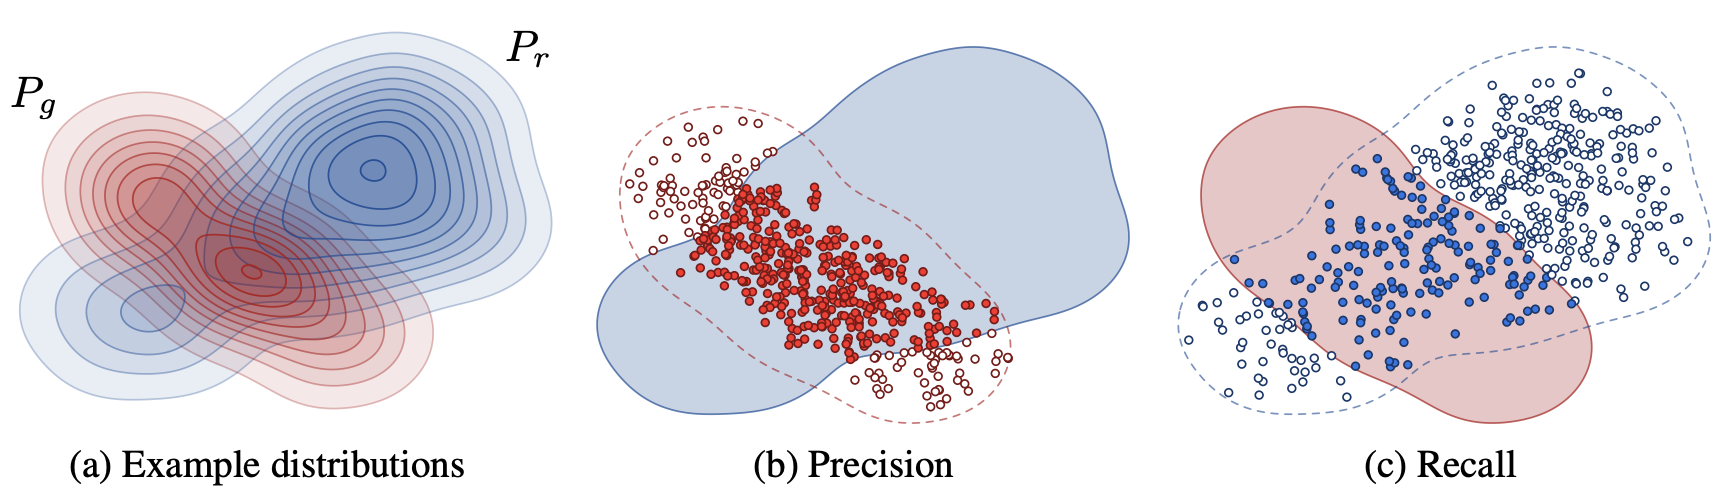
\includegraphics[width=0.95\linewidth]{figs/pr_curve}
	\end{figure}
	\vspace{-0.3cm}
	\begin{itemize}
		\item \textbf{Precision} denotes the fraction of generated images that are realistic.
		\item \textbf{Recall} measures the fraction of the training data manifold covered by the generator.
	\end{itemize}
	\myfootnotewithlink{https://arxiv.org/abs/1904.06991}{Kynkäänniemi T. et al. Improved precision and recall metric for assessing generative models, 2019}
\end{frame}
%=======
\begin{frame}{Precision-Recall}
	\vspace{-0.2cm}
	\begin{itemize}
		\item $\cS_{\pi} = \{\bx_i\}_{i=1}^{n} \sim \pi(\bx)$ -- real samples;
		\item $\cS_{p} = \{\bx_i\}_{i=1}^{n} \sim p(\bx | \btheta)$ -- generated samples.
	\end{itemize}
	Define binary function:
	\vspace{-0.2cm}
	\[
		\mathbb{I}(\bx, \cS) = 
		\begin{cases}
			1, \quad \text{if exists } \bx' \in \cS: \| \bx  - \bx'\|_2 \leq \| \bx' - \text{NN}_k(\bx', \cS)\|_2; \\
			0, \quad \text{otherwise.}
		\end{cases}
	\]
	\vspace{-0.3cm}
	\[
		\text{Precision} (\cS_{\pi}, \cS_{p}) = \frac{1}{n} \sum_{\mathbf{\bx} \in \cS_{p}} \mathbb{I}(\bx, \cS_{\pi}); \,\, \text{Recall} (\cS_{\pi}, \cS_{p}) = \frac{1}{n} \sum_{\bx \in \cS_{\pi}} \mathbb{I}(\bx, \cS_{p}).
	\]
	\vspace{-0.6cm}
	\begin{figure}
		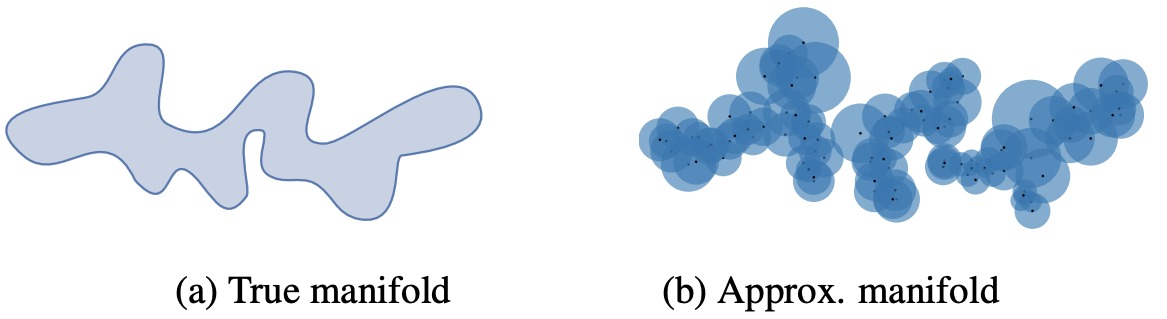
\includegraphics[width=0.75\linewidth]{figs/pr_k_nearest}
	\end{figure}
	Embed the samples using the pretrained network (as for FID).
	\myfootnotewithlink{https://arxiv.org/abs/1904.06991}{Kynkäänniemi T. et al. Improved precision and recall metric for assessing generative models, 2019}
\end{frame}
%=======
\begin{frame}{Precision-Recall}
	\begin{figure}
		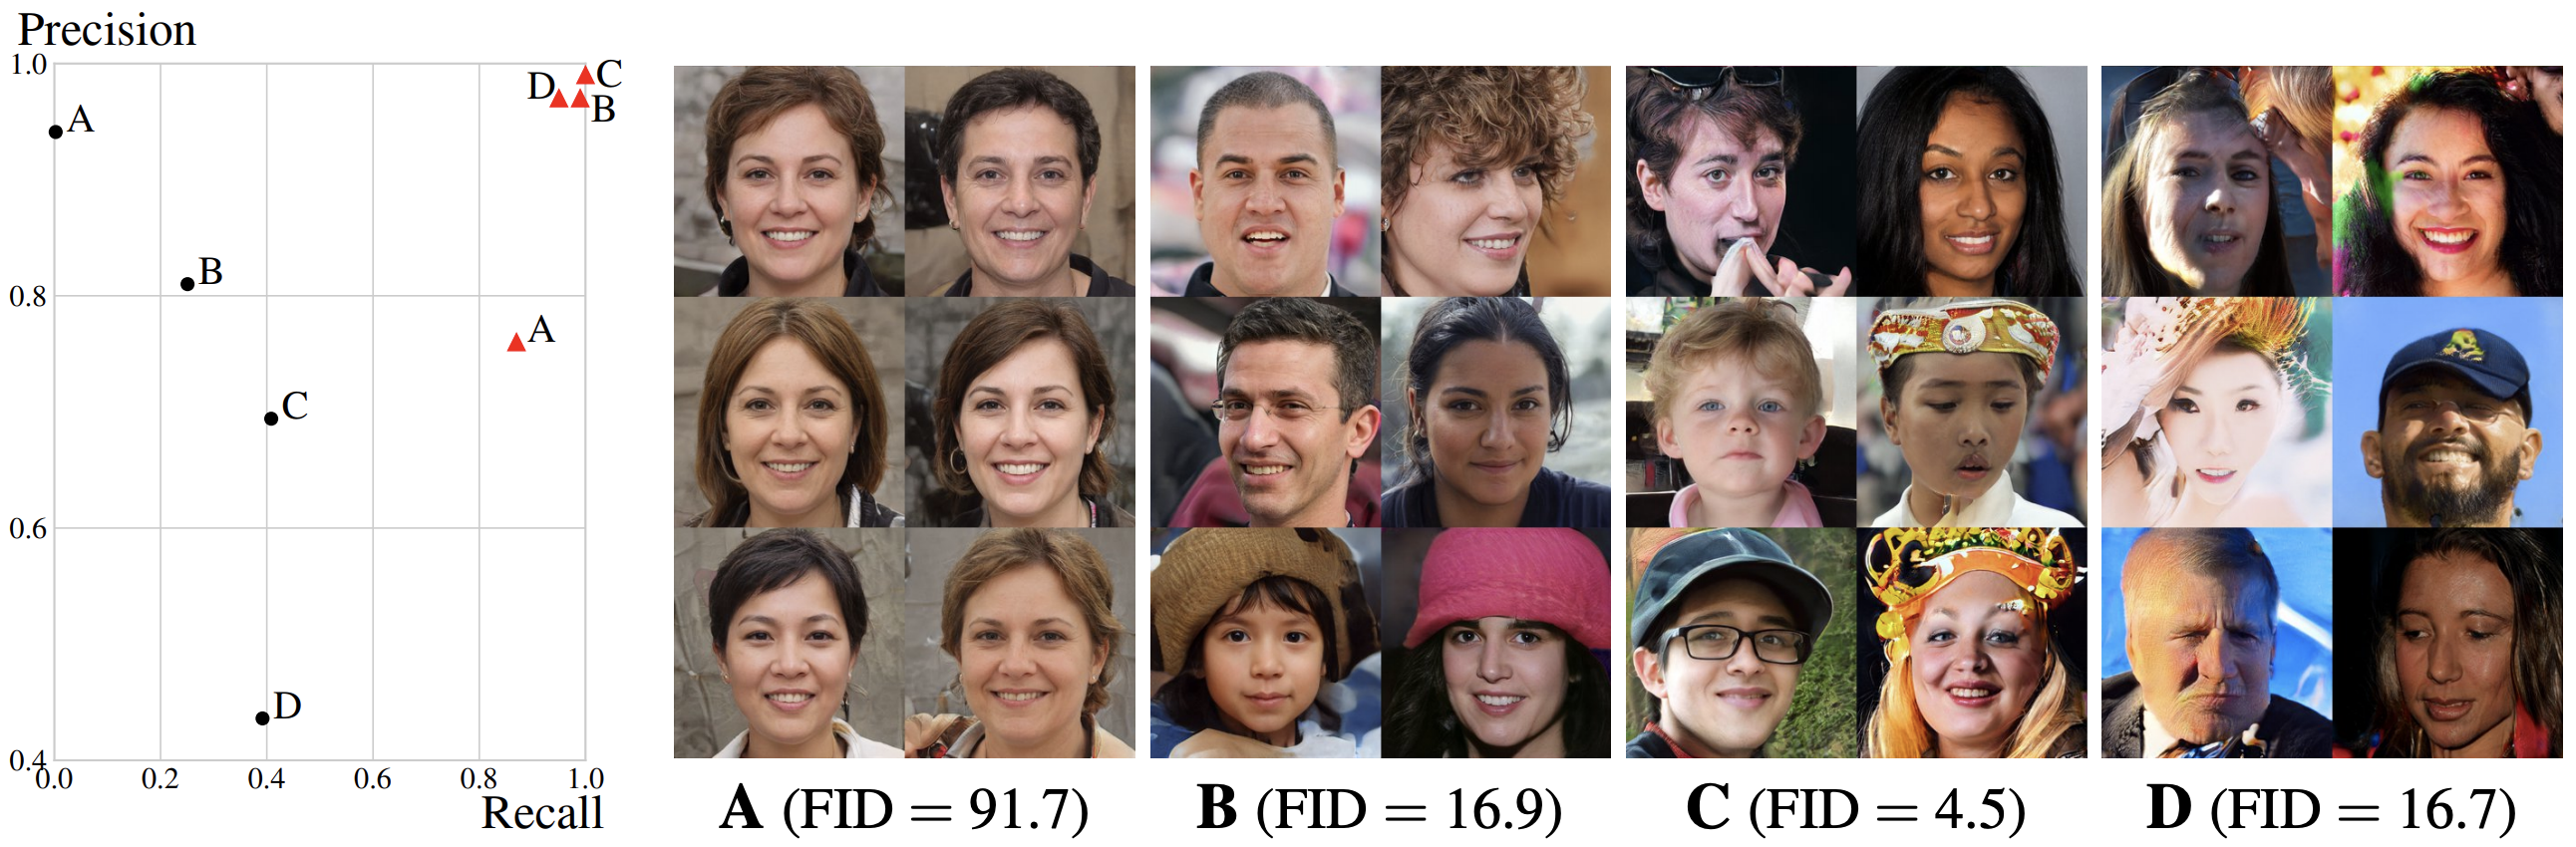
\includegraphics[width=\linewidth]{figs/pr_vs_fid}
	\end{figure}
	\begin{figure}
		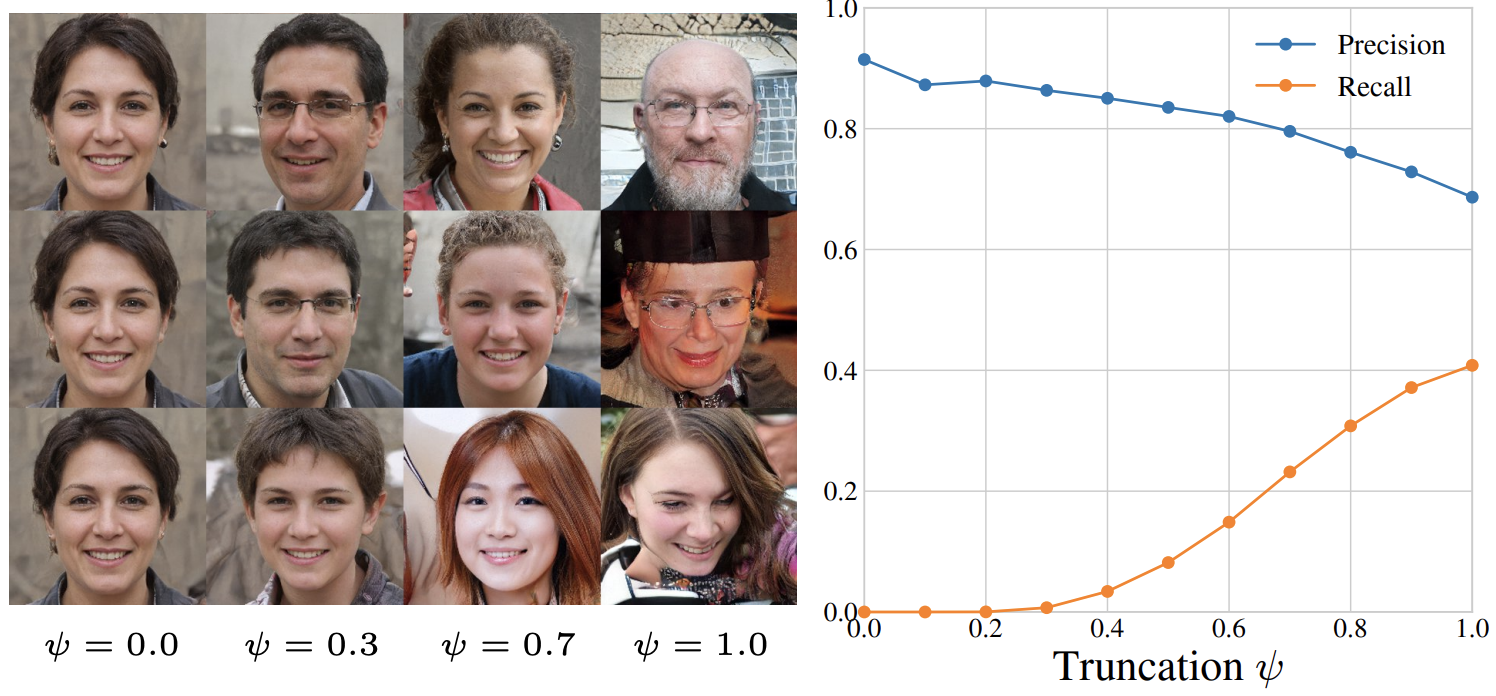
\includegraphics[width=0.75\linewidth]{figs/pr_truncation}
	\end{figure}
	\myfootnotewithlink{https://arxiv.org/abs/1904.06991}{Kynkäänniemi T. et al. Improved precision and recall metric for assessing generative models, 2019}
\end{frame}
%=======
\begin{frame}{Truncation trick}
	\begin{block}{BigGAN: truncated normal sampling}
		\[
			p(\bz | \psi) = \frac{\cN(\bz | 0, \bI)}{\int_{-\infty}^\psi \cN(\bz' | 0, \bI) d\bz'}
		\]
		Elements of $\bz \sim \cN(0, \bI)$ which fall outside a predefined range are resampled.
	\end{block}
	
	\begin{block}{StyleGAN}
		\vspace{-0.3cm}
		\[
			\bz' = \hat{\bz} + \psi \cdot (\bz - \hat{\bz}), \quad \hat{\bz} = \bbE_{\bz} \bz
		\]
		\vspace{-0.3cm}
		\begin{itemize}
			\item Constant $\psi$ is a tradeoff between diversity and fidelity. 
			\item $\psi=0.7$ is used for most of the results.
		\end{itemize}
	\end{block}

	\myfootnote{\href{https://arxiv.org/abs/1809.11096}{Brock A., Donahue J., Simonyan K. Large Scale GAN Training for High Fidelity Natural Image Synthesis, 2018} \\
	\href{https://arxiv.org/abs/1812.04948}{Karras T., Laine S., Aila T. A Style-Based Generator Architecture for Generative Adversarial Networks, 2018}}
\end{frame}
%=======
\begin{frame}{Summary}
	\begin{itemize}
		\item Kantorovich-Rubinstein duality gives the way to calculate the EM distance using only samples.
		\vfill
		\item Wasserstein GAN uses the weight clipping to ensure the Lipschitness of the critic.
		\vfill
		\item f-divergence family is a unified framework for divergence minimization, which uses variational approximation. Standard GAN is a special case of it.
		\vfill
		\item Frechet Inception Distance is the most popular metric for the implicit models evaluation. 
		\vfill
		\item Precision-recall allow to select model that compromises the sample quality and the sample diversity.	
		\vfill 
		\item Truncation tricks help to select model with the compromised samples: diverse and sharp.
	\end{itemize}
\end{frame}
\end{document} 